\documentclass[preview]{standalone}
\usepackage{amssymb, amsthm}
\usepackage[fleqn]{amsmath}

\usepackage{geometry}
%\geometry{paperwidth=12.5cm,margin=0mm}

\usepackage[no-math]{fontspec}
\usepackage{unicode-math}


%\setmainfont{GFS Neohellenic}
%\setmathfont{GFS Neohellenic Math}
%\usepackage{libertinus}
%\setsansfont{texgyreheros}[ 
%Extension = {.otf}, 
%UprightFont = {*-regular}, 
%ItalicFont = {*-italic}, 
%BoldFont = {*-bold}, 
%BoldItalicFont = {*-bolditalic}] 



\usepackage[no-math]{fontspec}
\usepackage{unicode-math}
\setmainfont{TeX Gyre Heros}
\setmathfont{Stix Two Math}

\usepackage{xcolor}
\definecolor{itwm_blue_04}{RGB}{0,90,148}
\definecolor{itwm_red}{RGB}{230,0,0}
\definecolor{background}{RGB}{249,249,249}

\usepackage{tikz}
\usepackage{pgfplots}
\pgfplotsset{compat=newest}
\usetikzlibrary{backgrounds}


\makeatletter
\tikzset{fixed ratio/.code={\def\tikz@pft##1:##2;{\edef\pgfutil@tempx{##1}\edef\pgfutil@tempy{##2}}%
    \expandafter\tikz@pft#1;%
    \tikzset{execute at end picture={%
    \ifcsname sa@border@right\endcsname
     \pgfmathsetmacro\pgfutil@tempa{((\pgf@picmaxx+\sa@border@right-\pgf@picminx+\sa@border@left)/%
     (\pgf@picmaxy+\sa@border@top-\pgf@picminy+\sa@border@bottom)}%
    \else
     \pgfmathsetmacro\pgfutil@tempa{((\pgf@picmaxx-\pgf@picminx)/(\pgf@picmaxy-\pgf@picminy)}%
    \fi
    \pgfmathsetmacro\pgfutil@tempb{(\pgfutil@tempx/\pgfutil@tempy)}%
    \ifdim\pgfutil@tempa pt=\pgfutil@tempb pt\relax
    \else
     \ifdim\pgfutil@tempb pt>\pgfutil@tempa pt\relax
      % target ratio greater than actual
      \pgfmathsetmacro\pgfutil@tempc{-(\pgf@picmaxx-\pgf@picminx)%
      +\pgfutil@tempb*(\pgf@picmaxy-\pgf@picminy)}%
      \path ([xshift=-0.5*\pgfutil@tempc]current bounding box.west)
       ([xshift=0.5*\pgfutil@tempc]current bounding box.east);
     \else
      % target ratio smaller than actual
      \pgfmathsetmacro\pgfutil@tempc{-(\pgf@picmaxy-\pgf@picminy)%
      +(\pgf@picmaxx-\pgf@picminx)/\pgfutil@tempb}%
      \path ([yshift=-0.5*\pgfutil@tempc]current bounding box.south)
       ([yshift=0.5*\pgfutil@tempc]current bounding box.north);
     \fi
    \fi
    }%  
    }}
}
\makeatother


\begin{document}
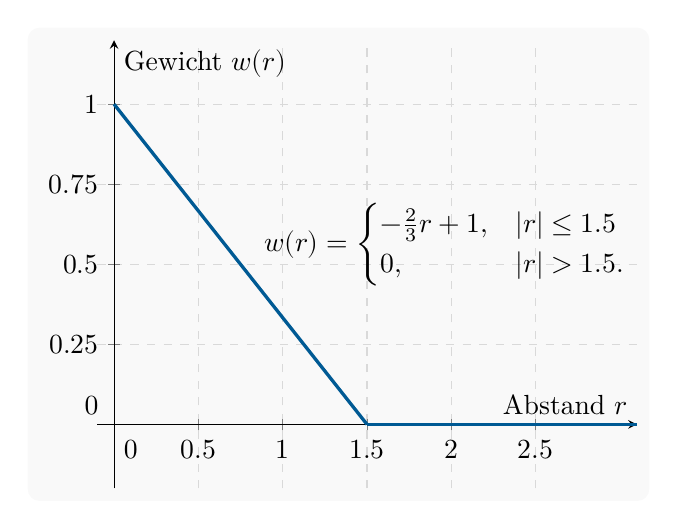
\begin{tikzpicture}[background rectangle/.style=
{fill=background,rounded corners=1ex}, show background rectangle]
\begin{axis}[
    axis lines = center,
    xlabel = {Abstand $r$},
    ylabel = {Gewicht $w(r)$},
    %height=8cm, width=12cm, 
    grid=major,
    grid style={dashed, gray!30},
    xmin=-.1, xmax=3.1, ymin=-.2, ymax=1.2,  
    xtick = {0, 0.5, ..., 2.5},
    ytick = {0, 0.25, ..., 1},
    after end axis/.code={
        \path (axis cs:0,0) 
            node [anchor=north west,yshift=-0.075cm] {0}
            node [anchor=south east,xshift=-0.075cm] {0};
    }
]
\addplot[draw=itwm_blue_04, smooth, very thick, domain=0:1.5]{-2/3*x+1};
\addplot[draw=itwm_blue_04, smooth, very thick, domain=1.5:3.1]{0};
\end{axis};
\node [anchor=west] (note) at (2,3.1) {$w(r)=\begin{cases}-\frac{2}{3} r+1, & |r|\leq 1.5\\ 0, &|r|>1.5. \end{cases}$};
\end{tikzpicture}

\end{document}